\documentclass[runningheads]{llncs}
\usepackage[spanish]{babel}
\usepackage[utf8]{inputenc}
\usepackage[T1]{fontenc}
\usepackage{graphicx}
\usepackage{amsmath}
\usepackage{amssymb}
\usepackage{hyperref}
\usepackage{wrapfig}
\usepackage{url}

\begin{document}

\title{PRISM: Verificación Formal de Sistemas con Modelos Probabilísticos}

\author{
    Angeles Carrara\and
    Julieta Paola Storino\and
    Mateo Carranza Velez}

\authorrunning{Carrara, Storino, Carranza-Velez}

\institute{
    Facultad de Matemática, Astronomía, Física y Computación.\\
    Universidad Nacional de Córdoba.
    \email{\{mateocvelez,julieta\_storino,angeles.carrara\}@mi.unc.edu.ar}}

\maketitle

\begin{abstract}
Este documento presenta un análisis general de la herramienta PRISM \cite{KNP11}, un entorno para el modelado y análisis formal de sistemas con comportamientos aleatorios o probabilísticos, que permite la verificación rigurosa de propiedades cuantitativas y cualitativas sobre modelos como cadenas de Markov (discretas y continuas), procesos de decisión de Markov y autómatas probabilísticos. Se abordan los principales aspectos relacionados con su desarrollo y aplicación, incluyendo: el contexto de creación de la herramienta, sus objetivos fundamentales, una descripción de sus funcionalidades desde la perspectiva del usuario, los componentes técnicos que la sustentan, casos de estudio documentados, una comparación con otras herramientas similares en el ámbito de la verificación formal y un análisis detallado de un caso de estudio seleccionado.
\end{abstract}

\section{Introducción}
Los sistemas informáticos se encuentran cada vez más integrados en múltiples áreas del conocimiento, enfrentando riesgos cada vez más críticos y de mayor impacto. Estos riesgos abarcan desde errores que pueden poner en peligro vidas humanas —como sobredosis de radiación provocadas por condiciones de carrera en sistemas médicos \cite{LT93}—, hasta pérdidas económicas multimillonarias —como autodestrucción en cohetes espaciales causado por conversión incorrecta de punto flotante a entero en sistemas de referencia inercial \cite{Lan96}—. Frente a esta realidad, se vuelve esencial garantizar sistemas más robustos, confiables y con tolerancia mínima al fallo. Para ello, es necesario recurrir a modelos formales que permitan describir con precisión las partes relevantes del sistema, conservando un nivel de abstracción que facilite su análisis y verificación.

\vspace{.5em}

\textsc{Organización del trabajo}. La Sección 2 presenta los conceptos teóricos necesarios para el uso de la herramienta. La Sección 3 describe su desarrollo y estado actual. Las Secciones 4 y 5 abordan la interfaz de usuario y los aspectos técnicos, respectivamente. En la Sección 6 se introducen dos casos de estudio, mientras que la Sección 7 ofrece una comparación con otras herramientas de verificación de modelos probabilísticos. La Sección 8 se dedica al modelado del problema de cruzar el río. Finalmente, el trabajo concluye con un resumen de los resultados obtenidos y una discusión sobre posibles líneas futuras de desarrollo.

\section{Antecedentes}
La verificación de modelos (model checking) es una técnica de verificación para la corrección funcional de un sistema. Consiste en explorar exhaustivamente todos los estados posibles del sistema con el objetivo de comprobar que cumple efectivamente con una propiedad cualitativa específica \cite{BK07}. La verificación de modelos probabilísticos (probabilistic model checking), por su parte, es una extensión que permite establecer la validez de una propiedad cuantitativa dentro de un modelo estocástico. Es diseñada para analizar sistemas que presentan comportamientos estocásticos, permitiendo obtener así valores como la probabilidad o el tiempo esperado hasta que ocurra un evento. Los principales modelos soportados por la herramienta a desarrollar son:

\vspace{.5em}

\textsc{Cadenas de Markov de Tiempo Discreto (DTMC)}: Modelan sistemas que evolucionan en pasos discretos, donde la probabilidad de transición al siguiente estado depende solo del estado actual. Se representan como grafos dirigidos, donde los nodos corresponden a los estados del sistema y las aristas están etiquetadas con probabilidades de transición.

\vspace{.5em}

\textsc{Cadenas de Markov de Tiempo Continuo (CTMC)}. Describen transiciones que ocurren tras un tiempo aleatorio continuo, regido por una distribución exponencial. Se representan mediante grafos dirigidos cuyas aristas están etiquetadas con tasas de transición, que definen el ritmo de cambio entre estados.

\vspace{.5em}

\textsc{Procesos de Decisión de Markov (MDP)}. Extienden las DTMC incorporando decisiones no deterministas. En cada estado hay varias acciones posibles, los cuales definen una distribución de probabilidad sobre los estados sucesores. Se representan como grafos con estructuras de decisión asociadas a cada estado.

\vspace{.5em}

Una vez que el sistema ha sido representado mediante un modelo, el siguiente paso es verificar si cumple con una especificación formal. Para ello, pueden emplearse diversos lenguajes de lógica temporal. Los principales lenguajes soportados por la herramienta a desarrollar son:

\vspace{.5em}

\textsc{Lógica de Árbol Computacional Probabilística (PCTL)}. Introducido por Hansson y Jonsson en \cite{HH94}, es una extensión probabilística de CTL que incorpora el operador $P$, el cual permite expresar propiedades sobre la probabilidad de ocurrencia de eventos en sistemas estocásticos. Por ejemplo, $a \to P_{\sim p}[F^{\le s} b]$ indica que, si ocurre $a$, entonces la probabilidad de que $b$ ocurra en los próximos $s$ pasos cumple la relación $\sim p$, donde $\sim\in\{>,\ge,<,\le\}$.

\vspace{.5em}

\textsc{Lógica Estocástica Continua (CSL)}: Introducida por Aziz et al. en \cite{ASSB96} y luego extendida por Baier et al. en \cite{BKH99}, es una extensión de PCTL que permite manejar tiempos de transición continuos entre estados. Sus operadores son similares, pero en lugar de valores discretos usan valores continuos. Además, CSL incorpora el operador de estado estacionario $S_{\sim p}[\phi]$, que expresa que la probabilidad de que la fórmula $\phi$ sea verdadera en el largo plazo cumple la relación $\sim p$. Por ejemplo, $a \to S_{\sim p}[b]$ indica que, si ocurre $a$, entonces la probabilidad de que $b$ ocurra en el largo plazo cumple la relación $\sim p$, donde $\sim\in\{>,\ge,<,\le\}$.

\section{Contexto de creación de la herramienta}
PRISM obtiene su nombre de \textit{Probabilistic (Symbolic) Model Checker} y es una herramienta de código abierto para la verificación de modelos probabilísticos. Su desarrollo comenzó en 1998 en la Universidad de Birmingham, su primer lanzamiento público oficial tuvo lugar en 2001 y en 2002 fue presentada formalmente como parte de la tesis doctoral de David Anthony Parker \cite{Par02}.

Además, sobre la base de PRISM, se desarrolló PRISM-games, una extensión presentada por primera vez en 2013, con versiones importantes en 2016 y 2020. Esta herramienta está orientada al análisis de juegos estocásticos multijugador, permitiendo modelar escenarios donde múltiples agentes interactúan de forma colaborativa o competitiva \cite{PRISMGames}. Si bien no se utiliza en este trabajo, se destaca como una evolución relevante del model checker original.

Hoy en día, el proyecto es mantenido activamente por el Departamento de Ciencias de la Computación de la Universidad de Oxford, con un repositorio actualizado en GitHub \cite{PRISMGitHub} y versiones disponibles para los sistemas operativos Linux, Windows, macOS y Solaris \cite{PRISMOxford}. Sus principales desarrolladores son David Parker, quien lidera el desarrollo del proyecto, y Marta Kwiatkowska (Universidad de Oxford) junto con Gethin Norman (Universidad de Glasgow) \cite{KNP09a}.

Hasta la fecha, se han documentado más de 400 casos de estudio utilizando PRISM en una extensa gama de dominios de aplicación \cite{KwiatkowskaEtaps2024}. Se emplea ampliamente en el ámbito académico, tanto en investigaciones independientes como en colaboraciones, y también ha sido aplicada en entornos industriales, particularmente en áreas críticas como los sistemas embebidos, los protocolos de comunicación y la seguridad.

Principalmente, se utiliza en las primeras etapas del desarrollo de sistemas, como la especificación, el diseño y la verificación formal, permitiendo la detección temprana de inconsistencias y errores. No obstante, también puede ser empleada en fases posteriores, como testing o mantenimiento, para validar propiedades del sistema o analizar modelos ya existentes.

\section{Descripción de la herramienta del lado del usuario}
Aunque PRISM puede utilizarse desde la línea de comandos, también cuenta con una interfaz gráfica compuesta por cuatro pestañas: \texttt{Model}, \texttt{Properties}, \texttt{Simulator} y \texttt{Log}, cada una con funciones específicas.

En la pestaña \texttt{Model} se especifica el tipo de modelo probabilístico a utilizar, que puede ser \texttt{dtmc}, \texttt{ctmc} y \texttt{mdp} entre otros. Un modelo —no confundir con los tipos mencionados— está compuesto por uno o más módulos. Cada módulo incluye variables que describen su estado y transiciones que dependen del estado actual del módulo y, posiblemente, del estado de otros módulos. En \texttt{dtmc} y \texttt{mpd}, cada transición especifica la probabilidad de pasar de un estado a otro, mientras que en \texttt{ctmc} se deben definir tasas en lugar de probabilidades.

En la pestaña \texttt{Properties} se definen las propiedades que se desean verificar mediante lógicas temporales probabilísticas, como \texttt{PCTL} y \texttt{CSL} entre otros. Estas propiedades pueden ser de dos tipos: unas son consultas booleanas que indican si una propiedad se cumple o no (por ejemplo, si la probabilidad de alcanzar un estado dado es al menos $0.5$); otras solicitan el cálculo de valores numéricos (como probabilidades específicas o tiempos esperados hasta que ocurra un evento). Para estos cálculos, se emplean las \textit{estructuras de costos y recompensas}, que pueden asignarse tanto a estados (\textit{state rewards}) como a transiciones (\textit{transition rewards}). Para más detalles sobre el lenguaje, consultar la documentación oficial \cite{PRISMManual}.

En la pestaña \texttt{Simulator} se pueden realizar simulaciones del modelo con una cantidad específica de pasos y transiciones, tanto aleatorias como manuales. Cuenta con una tabla de valores de las variables en cada paso y permite generar gráficos de las simulaciones realizadas. La pestaña \texttt{Log} contiene un reporte con las operaciones realizadas por PRISM, que incluye detalles técnicos como las estimaciones de los errores en los cálculos de probabilidades. 

La herramienta también permite visualizar los modelos, mediante la generación de archivos \textit{.dot} que contienen la información necesaria para dibujar los grafos asociados a estos. Con la herramienta \textit{GraphViz} podemos transformar estos archivos .dot a imágenes que muestren los grafos. La herramienta puede representar grafos de cualquier tamaño, es decir, no hay restricciones en la cantidad máxima de nodos o aristas. \footnote[1]{\href{https://github.com/marbl/MetagenomeScope/issues/28}{Issue de github que habla de esto}}

PRISM analiza principalmente propiedades cuantitativas y probabilísticas. Sin embargo, también es posible especificar propiedades no probabilísticas utilizando lógicas temporales como CTL. Cuando una propiedad de estas características no se cumple, en algunos casos la herramienta es capaz de generar contraejemplos que ilustran el comportamiento que lleva a dicha violación.

\section{Aspectos técnicos de la herramienta}
La herramienta toma como entrada la descripción de un sistema probabilístico escrito en el lenguaje PRISM\cite{KNP04b}\cite{Par02}, construye el modelo a partir de esta descripción, calcula el conjunto de estados alcanzables e identifica cualquier estado de bloqueo mutuo (deadlock).
A continuación, realiza la verificación del modelo para determinar qué estados del modelo cumplen cada especificación. Las estructuras de datos subyacentes en PRISM son \textit{Diagramas de Decisión Binaria} (BDD) y \textit{Diagramas de decisión binaria multi-terminal} (MTBDD). Sin embargo, para el cálculo numérico, la herramienta proporciona tres motores distintos que pueden utilizarse indistintamente. El primero es una implementación puramente basada en MTBDD; el segundo es una versión explícita convencional que utiliza matrices dispersas, implementada con fines comparativos; el tercero utiliza el enfoque híbrido.

Por otro lado, PRISM incorpora diversas técnicas de reducción para optimizar el análisis\cite{KNP11}. Por ejemplo, la reducción por simetría, que permite minimizar el número de estados únicos analizados, y la eliminación de estados inalcanzables mediante análisis de alcanzabilidad. También utiliza refinamiento cuantitativo de abstracciones, una técnica automática y extensible que construye y mejora sucesivamente modelos probabilísticos simplificados del sistema. Esta técnica se basa en la teoría de juegos y ha sido aplicada con éxito tanto a modelos temporizados como a MDP y software probabilístico, permitiendo una verificación escalable de sistemas grandes o infinitos.

La precisión de los resultados para propiedades cualitativas, como las de alcanzabilidad, es exacta. En cambio, para propiedades cuantitativas que requieren cálculos numéricos, como tiempos esperados, se utilizan métodos iterativos que aproximan la solución con una precisión configurable.

Finalmente, no se reportan falsos positivos ni negativos en sentido lógico. La posible inexactitud proviene del uso de métodos numéricos iterativos, los cuales podrían no alcanzar la precisión requerida si los parámetros de convergencia no están bien ajustados. Sin embargo, esto no compromete la corrección del enfoque algorítmico implementado por PRISM.

\section{Casos de estudio}
Se ha utilizado con éxito en el estudio de sistemas variados, incluyendo algoritmos distribuidos aleatorizados, protocolos de red, seguridad, procesos biológicos y teoría de juegos \cite{PRISMCaseStudies}. Se presentan brevemente dos casos de estudio:

\vspace{.5em}

\textsc{Bounded Retransmission Protocol (D'Argenio, Jeannet, Jensen \& Larsen)}\cite{PRISMBRP}:  Es un protocolo para enviar un archivo en partes, permitiendo un número limitado de reintentos por fragmento. Cuando no se logra transmitir un fragmento después de cierto número de intentos, se reporta un error. El modelo fue construido en PRISM como un DTMC. El sistema incluye módulos para el emisor, el receptor, un tester que controla el envío y dos canales con posibilidad de pérdida: uno para los mensajes y otro para los ACKs.

En el caso de estudio se analizaron varios tamaños del modelo. Utilizando 16 fragmentos ($N = 16$) y hasta 2 reintentos por fragmento ($MAX = 2$), los tiempos de verificación fueron bajos en todos los casos, con un máximo de $0.13$ segundos (fase de precómputo $+$ fase de algoritmo principal). El número de iteraciones necesarias varió según la propiedad verificada, alcanzando un máximo de 246 (también considerando ambas fases). Además, algunas propiedades se resolvieron en solo $0.001$ segundos mediante verificación de invariantes.

\vspace{.5em}

\textsc{Probabilistic Fair Exchange (Rabin)}\cite{PRISMFairExchange}: Se analiza el protocolo de Rabin para intercambio justo probabilístico entre dos partes asistidas por un tercero confiable. Las partes intercambian compromisos, condicionados a la publicación, en una fecha futura, de un número aleatorio entre 1 y $N$ por parte de un tercero. Si B envía el último mensaje, ambas partes quedan comprometidas con igual probabilidad; si lo hace A, hay una probabilidad de $1/N$ de que solo A lo esté. El protocolo se modeló como un MDP en PRISM, y el análisis confirmó que la probabilidad de estados injustos coincide con el valor teórico.

A modo ilustrativo, considérese un escenario en el que A se compromete a entregar un libro y B un disco, condicionados al sorteo de un número entre $1$ y $N$ en una fecha futura. Si el último mensaje enviado antes de dicha fecha fue de A, indicando un compromiso para el número $i+1$, y B no respondió, entonces existe una probabilidad $1/N$ de que el número sorteado sea exactamente $i+1$. En tal caso, A queda comprometida contractualmente y debe entregarle el libro a B, mientras que B no debe entregarle el disco a A, lo que evidencia un posible estado de injusticia inherente al protocolo.

El análisis en PRISM confirmó que la probabilidad máxima de alcanzar un estado injusto coincide con el valor teórico de $1/N$. Se verificó que los resultados coincidían exactamente con lo esperado: al usar $N = 10$, se obtuvo $0,1$; con $N = 100$, se obtuvo $0,01$; y con $N =1000$, se obtuvo $0,001$. Asimismo, se constató que la probabilidad de compromiso mutuo crece linealmente con el número de rondas de intercambio.

\section{Comparación con otras herramientas}
Hay muchas características de la herramienta que podemos destacar, basado en el reporte de la \textit{Comparación de herramientas para el análisis de datos cuantitativos} del 2019 \cite{Hahn2019}, donde se comparan modelos formales cuantitativos que capturan el comportamiento probabilístico, aspectos en tiempo real o dinámicas continuas generales.

Entre ellos, aunque de las cinco herramientas de propósito general presentadas —ePMC, mcsta, modes, PRISM y Storm— se destaca a Storm como la más versátil y, en cuanto a los formalismos que admiten, a PRISM y Storm como las que implementan la gama más amplia de propiedades, seguidas de ePMC. También se destaca a PRISM como la herramienta más usable, dada su extensa documentación en línea, una interfaz gráfica de usuario y descargas de binarios para todas las plataformas que solo dependen de Java.

Por otro lado, los resultados de la evaluación de rendimiento resaltan que PRISM y Storm pueden beneficiarse significativamente del uso de configuraciones no predeterminadas, ajustadas por expertos según los puntos de referencia individuales. mcsta muestra mejoras moderadas con un ajuste más simple.

También, dentro de muchas otras características presentadas por las distintas herramientas, los gráficos de cuantiles y dispersión muestran que Storm y PRISM lideran en velocidad y número de instancias resueltas, siendo Storm superior en configuraciones específicas. Sin embargo, todas las herramientas evaluadas fueron las más eficientes en ciertos casos particulares, y las especializadas resolvieron instancias únicas que otras no pudieron, cumpliendo su propósito. Casos como el modelo Haddad-Monmege expusieron limitaciones en precisión de ePMC, mcsta y PRISM bajo ciertas condiciones, mientras que la comparación entre configuraciones demostró que algunos errores o tiempos de espera pueden evitarse con ajustes adecuados, aunque esto no siempre es viable para usuarios comunes.

\section{Caso de estudio elegido: Cruzando el río probabilístico}
Para ilustrar el funcionamiento de la herramienta, vamos a modelar una versión probabilística del problema de ``cruzar el río'' \cite{Voolaid2007}, que es un acertijo lógico de la cultura popular, usado principalmente con fines de entretenimiento.

Un granjero quiere cruzar al otro lado del río junto con un lobo, una oveja y una lechuga. Para hacerlo, cuenta con un bote en el cual puede llevar, a lo sumo, un objeto. En cada momento, si hay $n$ objetos del lado del río en el que se encuentra, elige qué llevar de entre las $n+1$ opciones (nada o uno de los $n$ objetos) con igual probabilidad. Mientras el granjero está cruzando el río, si quedan del mismo lado el lobo junto con la oveja, la oveja junto con la lechuga o los tres, entonces alguien tiene probabilidad $p$ de ser devorado —la oveja, la lechuga y cualquiera de los dos con igual probabilidad respectivamente (pero en este último caso solo uno puede ser comido). Se busca entonces calcular la probabilidad de que el granjero pueda llegar al otro lado con los tres objetos.

Para lograr un modelado simple del problema\footnote[1]{\href{https://github.com/JulietaStorino/Software-Engineering-II-FAMAF/blob/main/caso_estudio/crossing.pm}{Link al repositorio}} usamos que, en PRISM, el no determinismo en una DTMC se traduce a una transición aleatoria con igual probabilidad entre todas las opciones posibles en ese momento. No incluiremos su grafo, pues tiene 72 estados y 124 transiciones.

En las formulaciones usuales del problema, siempre que alguien pueda ser comido, lo será, es decir, $p=1$. En esa versión, la probabilidad de cruzar exitosamente el río es de $0.006$ (o sea, $0.6\%$). Además, calculamos cómo varía la probabilidad de cruzar exitosamente para valores de $p$ entre 0 y 1, con saltos de a $0.1$ (figura 1). También calculamos cómo varía la probabilidad de cruzar exitosamente con $p=0.5$ y con cantidades de pasos entre 0 y 100 (figura 2). En el segundo caso, podemos notar que se forman \textit{mesetas} debido a que solo cada 4 pasos el granjero llega al lado derecho del río, lo que genera saltos discretos en la probabilidad de éxito.

\begin{figure}
  \centering
  \text{\textbf{Figura 1} (izq.) y \textbf{Figura 2} (der.)}
  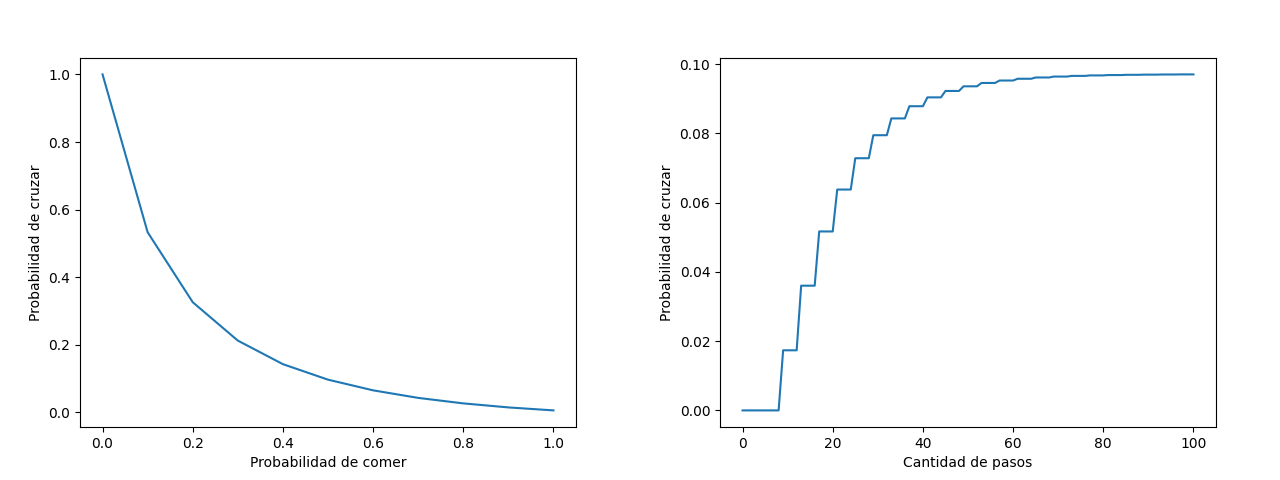
\includegraphics[width=12cm]{graficos.png}
\end{figure}

Verificamos las propiedades ``Con probabilidad 1, en algún momento se comen a la oveja'' y ``En algún momento se comen a la oveja'' —la primera es probabilística y la segunda no— obteniendo que la primera resulta verdadera, pero la segunda resulta falsa. Esto es porque existe un camino infinito en el que no se comen a la oveja, pero este tiene probabilidad 0 de ocurrir. PRISM no reporta contraejemplos en estos casos infinitos. Si en cambio verificamos la propiedad ``Pueden cruzar todos al otro lado'' (que tampoco es probabilística), esto resulta verdadero y PRISM nos da el testigo de cómo hacerlo mediante el simulador.

Por último, usando el sistema de recompensas de PRISM, calculamos el valor esperado de ``la cantidad de cruces que ocurren hasta que se comen a alguien'' y ``la cantidad de cruces que ocurren hasta resolver el problema o hasta que el problema no se puede resolver'' —porque se comieron a alguien. Para $p=0.5$, estos valores dieron aproximadamente $6.15$ y $5.55$ cruces respectivamente.

\section{Conclusiones}
PRISM se destaca en el ámbito de verificación de modelos probabilísticos, para el cual fue desarrollado, por su equilibrio entre usabilidad, amplitud de funcionalidades y buen rendimiento en una amplia variedad de instancias. Su documentación extensa, interfaz gráfica y disponibilidad multiplataforma la hacen especialmente accesible para usuarios no expertos, mientras que su capacidad para seleccionar motores de análisis eficientes por instancia le permite mantener un rendimiento competitivo frente a herramientas más recientes.

Por nuestra parte, la herramienta nos resultó bastante fácil de instalar y de utilizar. Esto se debe a que el manual \cite{PRISMManual} es de fácil lectura y es muy didáctico. Los modelos de ejemplo que trae también fueron de gran ayuda.

En un posible trabajo futuro, sería interesante modelar otros problemas clásicos similares al abordado en este trabajo, como por ejemplo el de \textit{los esposos celosos} o el de \textit{los misioneros y los caníbales}\cite{Efimova2018}, dado que ofrecen desafíos adicionales en cuanto a la representación de restricciones lógicas. También se podría extender el análisis modelando el mismo problema presentado utilizando los distintos tipos de modelos disponibles en PRISM con el fin de comparar resultados, capacidades de modelado y tiempos de verificación entre enfoques discretos, continuos y no deterministas.

\newpage

\begin{thebibliography}{21}

\bibitem{KNP11}
Kwiatkowska, M., Norman, G., Parker, D.: PRISM 4.0: Verification of Probabilistic Real-time Systems. In: Gopalakrishnan, G., Qadeer, S. (eds.) CAV 2011. LNCS, vol. 6806, pp. 585--591. Springer, Heidelberg (2011)

\bibitem{LT93}
Leveson, N.G., Turner, C.S.: An Investigation of the Therac-25 Accidents. IEEE Computer 26(7), 18--41 (1993)

\bibitem{Lan96}
Le Lann, G.: The Ariane 5 Flight 501 Failure -- A Case Study in System Engineering for Computing Systems. Rapport de recherche 3079 (1996)

\bibitem{BK07}
Baier, C., Katoen, J.-P.: Principles of Model Checking. MIT Press, Cambridge (2007)

\bibitem{KNP02}
Kwiatkowska, M., Norman, G., Parker, D.: PRISM: Probabilistic Symbolic Model Checker. In: Field, T., Harrison, P.G., Bradley, J.T., Harder, U. (eds.) TOOLS 2002. LNCS, vol. 2324, pp. 200--204. Springer, Heidelberg (2002)

\bibitem{HH94}
Hansson, H., Jonsson, B.: A Logic for Reasoning about Time and Probability. Formal Aspects of Computing 6(5), 512--535 (1994)

\bibitem{ASSB96}
Aziz, A., Sanwal, K., Singhal, V., Brayton, R.: Verifying Continuous Time Markov Chains. In: CAV 1996. LNCS, vol. 1102, pp. 269--276. Springer, Heidelberg (1996)

\bibitem{BKH99}
Baier, C., Katoen, J.-P., Hermanns, H.: Approximate Symbolic Model Checking of Continuous-Time Markov Chains. In: CONCUR 1999. LNCS, vol. 1664, pp. 146--161. Springer, Heidelberg (1999)

\bibitem{Par02}
Parker, D.: Implementation of Symbolic Model Checking for Probabilistic Systems. PhD thesis, University of Birmingham (2002)

\bibitem{PRISMGames}
\href{https://www.prismmodelchecker.org/games/}{PRISM Model Checker: PRISM-games.} Último acceso: junio 2025.

\bibitem{PRISMGitHub}
\href{https://github.com/prismmodelchecker/prism/blob/master/README.md}{PRISM Model Checker – GitHub Repository. README file.} Último acceso: mayo 2025.

\bibitem{PRISMOxford}
\href{https://www.cs.ox.ac.uk/activities/prism/}{PRISM Model Checker – University of Oxford.} Último acceso: mayo 2025.

\bibitem{KNP09a}
Kwiatkowska, M., Norman, G., Parker, D.: PRISM: Probabilistic Model Checking for Performance and Reliability Analysis. ACM SIGMETRICS Performance Evaluation Review 36(4), 40--45 (2009)

\bibitem{KwiatkowskaEtaps2024}
Kwiatkowska, M. (2024, abril). PRISM: ETAPS Test-of-Time Tool Award 2024 [Presentación de conferencia]. European Joint Conferences on Theory and Practice of Software (ETAPS 2024), Luxemburgo.

\bibitem{PRISMManual}
\href{https://www.prismmodelchecker.org/manual/Main/AllOnOnePage}{PRISM Model Checker. PRISM Manual.} Último acceso: mayo 2025.

\bibitem{KNP04b}
Kwiatkowska, M., Norman, G., Parker, D.: Probabilistic Symbolic Model Checking with PRISM: A Hybrid Approach. International Journal on Software Tools for Technology Transfer (STTT) 6(2), 128--142 (2004)

\bibitem{PRISMCaseStudies}
\href{https://www.prismmodelchecker.org/casestudies/index.php}{PRISM Model Checker: Case Studies Index.} Último acceso: mayo 2025.

\bibitem{PRISMBRP}
\href{https://www.prismmodelchecker.org/casestudies/brp.php}{PRISM Model Checker: Case Study – Bounded Retransmission Protocol (BRP).} Último acceso: mayo 2025.

\bibitem{PRISMFairExchange}
\href{https://www.prismmodelchecker.org/casestudies/fairexchange.php}{PRISM Model Checker: Case Study – Probabilistic Fair Exchange.} Último acceso: mayo 2025.

\bibitem{Hahn2019}
Hahn, E. M., Hartmanns, A., Hensel, C., Klauck, M., Klein, J., Kretínský, J., Parker, D., Quatmann, T., Ruijters, E., Steinmetz, M.: The 2019 comparison of tools for the analysis of quantitative formal models - (QComp 2019 competition report). In: TACAS (3), LNCS, vol. 11429, pp. 69–92. Springer (2019)

\bibitem{Voolaid2007}
Voolaid, Piret. (2007). Carrying a Wolf, a Goat, and a Cabbage across the Stream. Metamorphoses of ATU 1579. Folklore (Tartu). 35. 10.7592/FEJF2007.35.voolaid. 

\bibitem{Efimova2018}
Efimova, Elena. (2018). River Crossing Problems: Algebraic Approach.

\end{thebibliography}
\end{document}
